\documentclass{standalone}
\usepackage{tikz}
\usetikzlibrary{patterns, positioning}
\usepackage[sfdefault]{ClearSans} %% option 'sfdefault' activates Clear Sans as the default text font
\usepackage[T1]{fontenc}

\begin{document}
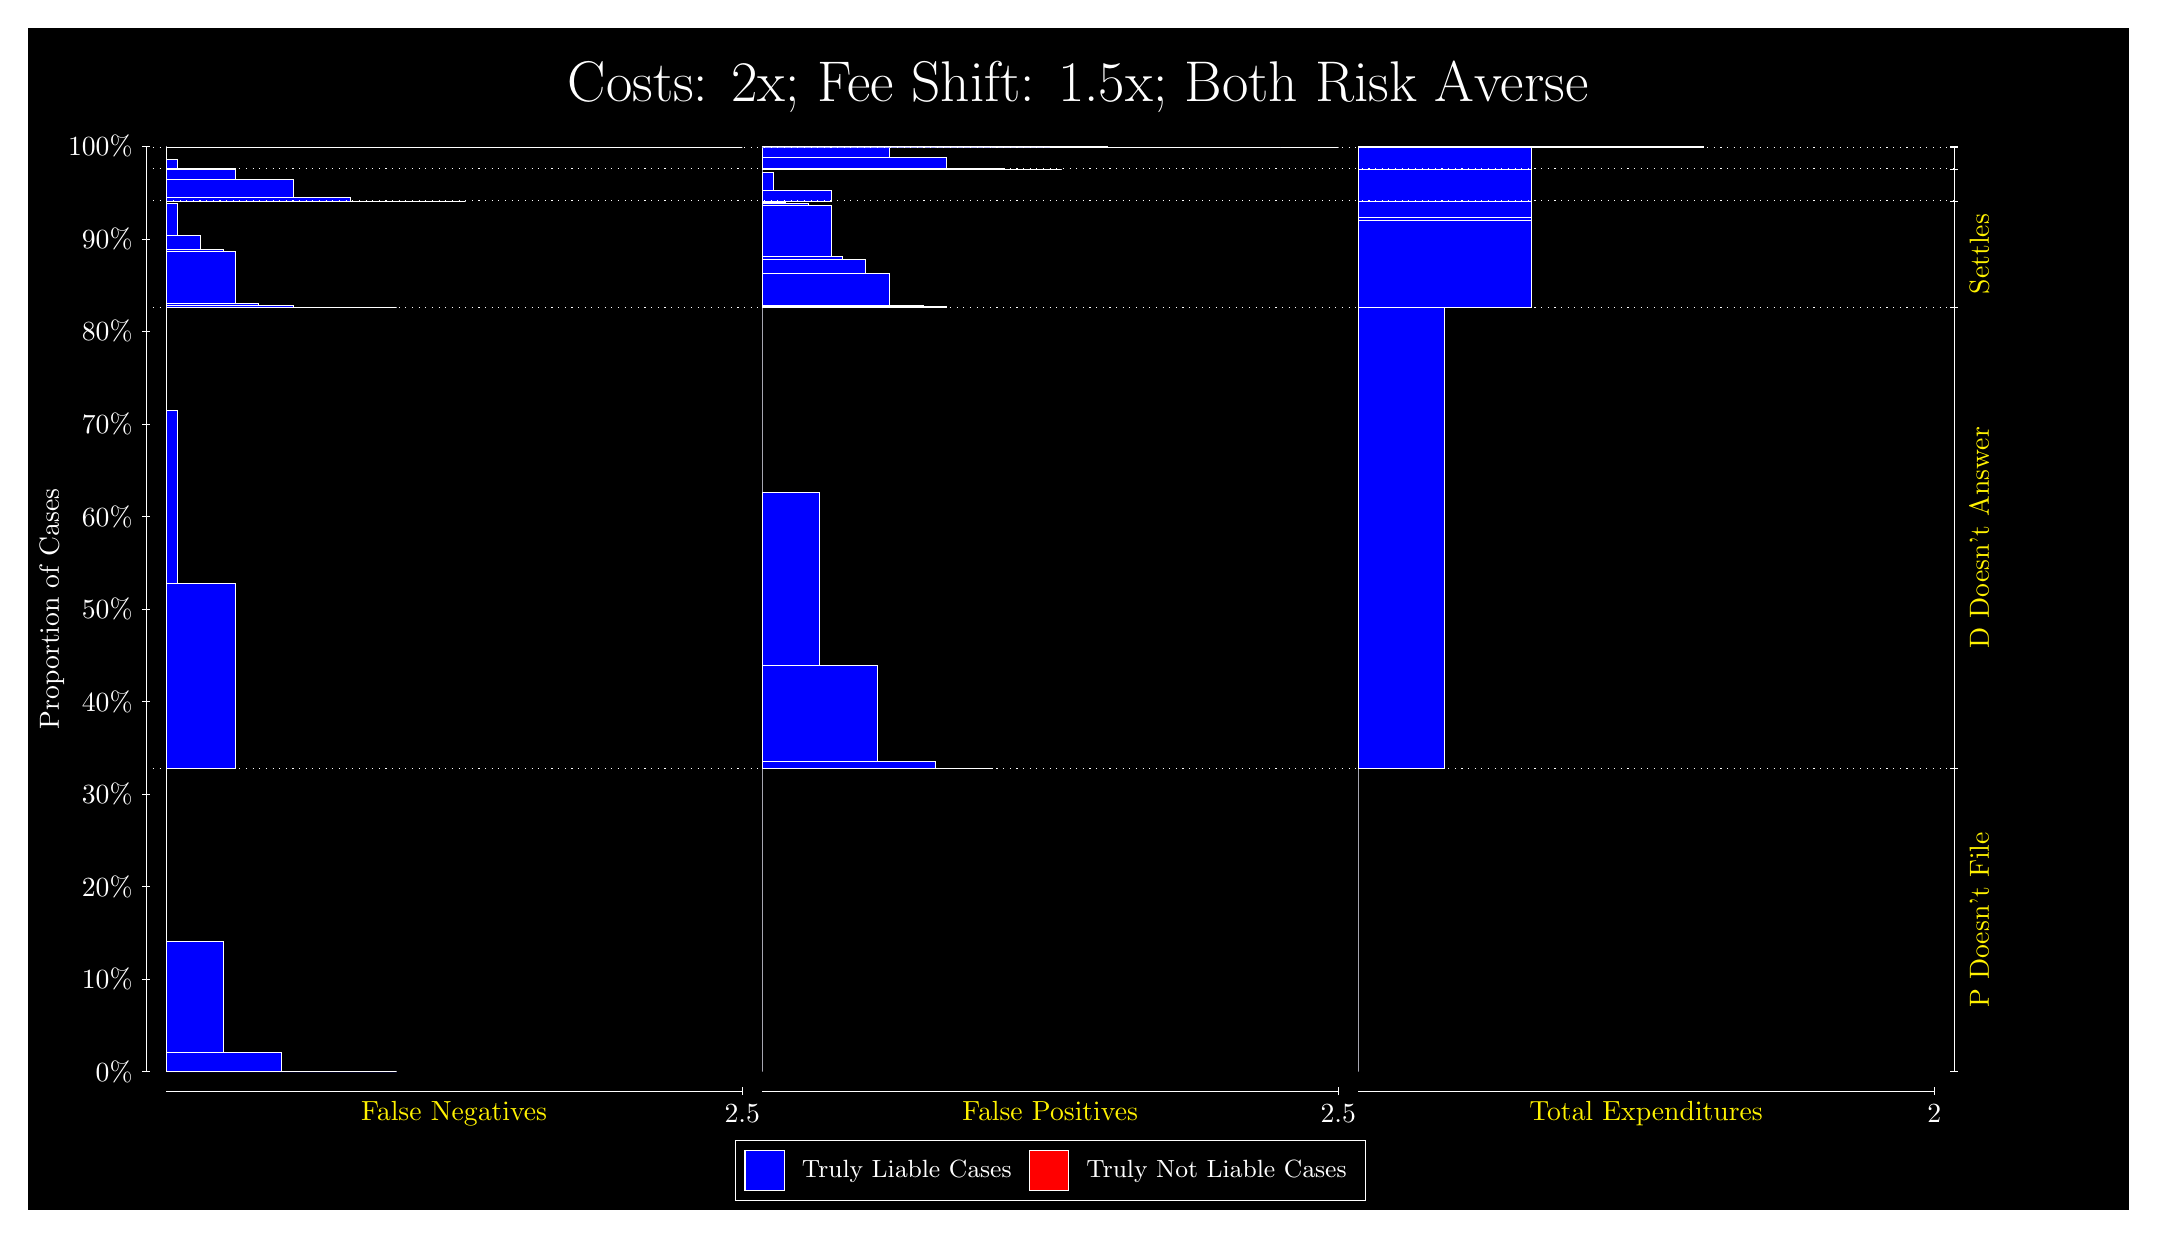
\begin{tikzpicture}
\draw[fill=black] (0,0) rectangle (26.667,15);
\draw[text=white] (0,13.5) rectangle (26.667,15) node[midway] {\huge Costs: 2x; Fee Shift: 1.5x; Both Risk Averse};
\draw[white, very thin] (1.5,1.75) -- (1.5,13.5);
\node[rotate=90, text=white, anchor=center] at (0.3, 7.625) {Proportion of Cases};
\draw[white, very thin] (1.45,1.75) -- (1.55,1.75);
\node[text=white, anchor=east] at (1.45, 1.75) {0\%};
\draw[white, very thin] (1.45,2.925) -- (1.55,2.925);
\node[text=white, anchor=east] at (1.45, 2.925) {10\%};
\draw[white, very thin] (1.45,4.1) -- (1.55,4.1);
\node[text=white, anchor=east] at (1.45, 4.1) {20\%};
\draw[white, very thin] (1.45,5.275) -- (1.55,5.275);
\node[text=white, anchor=east] at (1.45, 5.275) {30\%};
\draw[white, very thin] (1.45,6.45) -- (1.55,6.45);
\node[text=white, anchor=east] at (1.45, 6.45) {40\%};
\draw[white, very thin] (1.45,7.625) -- (1.55,7.625);
\node[text=white, anchor=east] at (1.45, 7.625) {50\%};
\draw[white, very thin] (1.45,8.8) -- (1.55,8.8);
\node[text=white, anchor=east] at (1.45, 8.8) {60\%};
\draw[white, very thin] (1.45,9.975) -- (1.55,9.975);
\node[text=white, anchor=east] at (1.45, 9.975) {70\%};
\draw[white, very thin] (1.45,11.15) -- (1.55,11.15);
\node[text=white, anchor=east] at (1.45, 11.15) {80\%};
\draw[white, very thin] (1.45,12.325) -- (1.55,12.325);
\node[text=white, anchor=east] at (1.45, 12.325) {90\%};
\draw[white, very thin] (1.45,13.5) -- (1.55,13.5);
\node[text=white, anchor=east] at (1.45, 13.5) {100\%};

\draw[white, very thin] (24.457,1.75) -- (24.457,13.5);
\draw[white, very thin] (24.407,1.75) -- (24.507,1.75);
\node[anchor=west] at (24.407, 1.75) {};
\draw[white, very thin] (24.407,5.6001) -- (24.507,5.6001);
\node[anchor=west] at (24.407, 5.6001) {};
\draw[white, very thin] (24.407,11.455) -- (24.507,11.455);
\node[anchor=west] at (24.407, 11.455) {};
\draw[white, very thin] (24.407,12.807) -- (24.507,12.807);
\node[anchor=west] at (24.407, 12.807) {};
\draw[white, very thin] (24.407,13.214) -- (24.507,13.214);
\node[anchor=west] at (24.407, 13.214) {};
\draw[white, very thin] (24.407,13.488) -- (24.507,13.488);
\node[anchor=west] at (24.407, 13.488) {};
\draw[white, very thin] (24.407,13.5) -- (24.507,13.5);
\node[anchor=west] at (24.407, 13.5) {};

\draw[white, very thin, fill=blue] (1.75,1.75) rectangle (4.6775,1.75);
\draw[white, very thin, fill=blue] (1.75,1.75) rectangle (3.9457,1.7521);
\draw[white, very thin, fill=blue] (1.75,1.7521) rectangle (3.2138,1.9952);
\draw[white, very thin, fill=blue] (1.75,1.9952) rectangle (2.4819,3.408);
\draw[white, very thin, fill=red] (1.75,3.408) rectangle (1.75,3.408);
\draw[white, very thin, fill=blue] (1.75,3.408) rectangle (1.75,5.6001);
\draw[white, very thin, fill=blue] (1.75,5.6001) rectangle (2.6283,7.9485);
\draw[white, very thin, fill=blue] (1.75,7.9485) rectangle (1.8964,10.15);
\draw[white, very thin, fill=red] (1.75,10.15) rectangle (1.75,10.15);
\draw[white, very thin, fill=blue] (1.75,10.15) rectangle (1.75,11.455);
\draw[white, very thin, fill=blue] (1.75,11.455) rectangle (4.6775,11.455);
\draw[white, very thin, fill=blue] (1.75,11.455) rectangle (4.3848,11.455);
\draw[white, very thin, fill=blue] (1.75,11.455) rectangle (4.092,11.455);
\draw[white, very thin, fill=blue] (1.75,11.455) rectangle (3.9457,11.455);
\draw[white, very thin, fill=blue] (1.75,11.455) rectangle (3.6529,11.455);
\draw[white, very thin, fill=blue] (1.75,11.455) rectangle (3.3602,11.478);
\draw[white, very thin, fill=blue] (1.75,11.478) rectangle (3.2138,11.48);
\draw[white, very thin, fill=blue] (1.75,11.48) rectangle (2.921,11.505);
\draw[white, very thin, fill=blue] (1.75,11.505) rectangle (2.6283,12.164);
\draw[white, very thin, fill=blue] (1.75,12.164) rectangle (2.4819,12.198);
\draw[white, very thin, fill=blue] (1.75,12.198) rectangle (2.1891,12.37);
\draw[white, very thin, fill=blue] (1.75,12.37) rectangle (1.8964,12.78);
\draw[white, very thin, fill=red] (1.75,12.78) rectangle (1.75,12.78);
\draw[white, very thin, fill=blue] (1.75,12.78) rectangle (1.75,12.807);
\draw[white, very thin, fill=blue] (1.75,12.807) rectangle (5.5558,12.807);
\draw[white, very thin, fill=blue] (1.75,12.807) rectangle (4.8239,12.807);
\draw[white, very thin, fill=blue] (1.75,12.807) rectangle (4.092,12.856);
\draw[white, very thin, fill=blue] (1.75,12.856) rectangle (3.3602,13.083);
\draw[white, very thin, fill=blue] (1.75,13.083) rectangle (2.6283,13.214);
\draw[white, very thin, fill=red] (1.75,13.214) rectangle (1.75,13.214);
\draw[white, very thin, fill=blue] (1.75,13.214) rectangle (2.6283,13.215);
\draw[white, very thin, fill=blue] (1.75,13.215) rectangle (1.8964,13.339);
\draw[white, very thin, fill=red] (1.75,13.339) rectangle (1.75,13.339);
\draw[white, very thin, fill=blue] (1.75,13.339) rectangle (1.75,13.488);
\draw[white, very thin, fill=blue] (1.75,13.488) rectangle (9.0689,13.488);
\draw[white, very thin, fill=blue] (1.75,13.488) rectangle (8.337,13.488);
\draw[white, very thin, fill=blue] (1.75,13.488) rectangle (7.6051,13.488);
\draw[white, very thin, fill=blue] (1.75,13.488) rectangle (6.8732,13.491);
\draw[white, very thin, fill=blue] (1.75,13.491) rectangle (6.1413,13.491);
\draw[white, very thin, fill=blue] (1.75,13.491) rectangle (5.4094,13.491);
\draw[white, very thin, fill=blue] (1.75,13.491) rectangle (3.0674,13.491);
\draw[white, very thin, fill=blue] (1.75,13.491) rectangle (2.3355,13.491);
\draw[white, very thin, fill=red] (1.75,13.491) rectangle (1.75,13.491);
\draw[white, very thin, fill=blue] (1.75,13.491) rectangle (1.75,13.5);
\draw[white, very thin, fill=red] (9.3189,1.75) rectangle (9.3189,1.75);
\draw[white, very thin, fill=blue] (9.3189,1.75) rectangle (9.3189,5.6001);
\draw[white, very thin, fill=red] (9.3189,5.6001) rectangle (12.246,5.6001);
\draw[white, very thin, fill=blue] (9.3189,5.6001) rectangle (12.246,5.6002);
\draw[white, very thin, fill=blue] (9.3189,5.6002) rectangle (11.515,5.6917);
\draw[white, very thin, fill=blue] (9.3189,5.6917) rectangle (10.783,6.9052);
\draw[white, very thin, fill=blue] (9.3189,6.9052) rectangle (10.051,9.1062);
\draw[white, very thin, fill=blue] (9.3189,9.1062) rectangle (9.3189,11.455);
\draw[white, very thin, fill=red] (9.3189,11.455) rectangle (11.661,11.455);
\draw[white, very thin, fill=blue] (9.3189,11.455) rectangle (11.661,11.467);
\draw[white, very thin, fill=red] (9.3189,11.467) rectangle (11.368,11.467);
\draw[white, very thin, fill=blue] (9.3189,11.467) rectangle (11.368,11.479);
\draw[white, very thin, fill=red] (9.3189,11.479) rectangle (11.075,11.479);
\draw[white, very thin, fill=blue] (9.3189,11.479) rectangle (11.075,11.482);
\draw[white, very thin, fill=blue] (9.3189,11.482) rectangle (10.929,11.892);
\draw[white, very thin, fill=blue] (9.3189,11.892) rectangle (10.636,12.064);
\draw[white, very thin, fill=blue] (9.3189,12.064) rectangle (10.344,12.098);
\draw[white, very thin, fill=blue] (9.3189,12.098) rectangle (10.197,12.757);
\draw[white, very thin, fill=blue] (9.3189,12.757) rectangle (9.9044,12.782);
\draw[white, very thin, fill=blue] (9.3189,12.782) rectangle (9.6116,12.784);
\draw[white, very thin, fill=blue] (9.3189,12.784) rectangle (9.4652,12.807);
\draw[white, very thin, fill=blue] (9.3189,12.807) rectangle (9.3189,12.807);
\draw[white, very thin, fill=red] (9.3189,12.807) rectangle (10.197,12.807);
\draw[white, very thin, fill=blue] (9.3189,12.807) rectangle (10.197,12.938);
\draw[white, very thin, fill=blue] (9.3189,12.938) rectangle (9.4652,13.165);
\draw[white, very thin, fill=blue] (9.3189,13.165) rectangle (9.3189,13.214);
\draw[white, very thin, fill=red] (9.3189,13.214) rectangle (13.125,13.214);
\draw[white, very thin, fill=blue] (9.3189,13.214) rectangle (13.125,13.214);
\draw[white, very thin, fill=blue] (9.3189,13.214) rectangle (12.393,13.216);
\draw[white, very thin, fill=blue] (9.3189,13.216) rectangle (11.661,13.363);
\draw[white, very thin, fill=blue] (9.3189,13.363) rectangle (10.929,13.486);
\draw[white, very thin, fill=blue] (9.3189,13.486) rectangle (10.197,13.488);
\draw[white, very thin, fill=red] (9.3189,13.488) rectangle (16.638,13.488);
\draw[white, very thin, fill=blue] (9.3189,13.488) rectangle (16.638,13.488);
\draw[white, very thin, fill=red] (9.3189,13.488) rectangle (15.906,13.488);
\draw[white, very thin, fill=blue] (9.3189,13.488) rectangle (15.906,13.488);
\draw[white, very thin, fill=red] (9.3189,13.488) rectangle (15.174,13.488);
\draw[white, very thin, fill=blue] (9.3189,13.488) rectangle (15.174,13.488);
\draw[white, very thin, fill=red] (9.3189,13.488) rectangle (14.442,13.488);
\draw[white, very thin, fill=blue] (9.3189,13.488) rectangle (14.442,13.491);
\draw[white, very thin, fill=blue] (9.3189,13.491) rectangle (13.71,13.497);
\draw[white, very thin, fill=blue] (9.3189,13.497) rectangle (12.978,13.497);
\draw[white, very thin, fill=blue] (9.3189,13.497) rectangle (12.246,13.497);
\draw[white, very thin, fill=blue] (9.3189,13.497) rectangle (11.515,13.497);
\draw[white, very thin, fill=red] (9.3189,13.497) rectangle (9.3189,13.497);
\draw[white, very thin, fill=blue] (9.3189,13.497) rectangle (9.3189,13.5);
\draw[white, very thin, fill=red] (16.888,1.75) rectangle (16.888,1.75);
\draw[white, very thin, fill=blue] (16.888,1.75) rectangle (16.888,5.6001);
\draw[white, very thin, fill=red] (16.888,5.6001) rectangle (17.986,5.6001);
\draw[white, very thin, fill=blue] (16.888,5.6001) rectangle (17.986,11.455);
\draw[white, very thin, fill=red] (16.888,11.455) rectangle (19.083,11.455);
\draw[white, very thin, fill=blue] (16.888,11.455) rectangle (19.083,12.56);
\draw[white, very thin, fill=red] (16.888,12.56) rectangle (19.083,12.56);
\draw[white, very thin, fill=blue] (16.888,12.56) rectangle (19.083,12.598);
\draw[white, very thin, fill=red] (16.888,12.598) rectangle (19.083,12.598);
\draw[white, very thin, fill=blue] (16.888,12.598) rectangle (19.083,12.807);
\draw[white, very thin, fill=red] (16.888,12.807) rectangle (19.083,12.807);
\draw[white, very thin, fill=blue] (16.888,12.807) rectangle (19.083,13.214);
\draw[white, very thin, fill=red] (16.888,13.214) rectangle (19.083,13.214);
\draw[white, very thin, fill=blue] (16.888,13.214) rectangle (19.083,13.488);
\draw[white, very thin, fill=red] (16.888,13.488) rectangle (21.279,13.488);
\draw[white, very thin, fill=blue] (16.888,13.488) rectangle (21.279,13.5);
\draw[white, dotted] (1.5,5.6001) -- (24.457,5.6001);
\draw[white, dotted] (1.5,11.455) -- (24.457,11.455);
\draw[white, dotted] (1.5,12.807) -- (24.457,12.807);
\draw[white, dotted] (1.5,13.214) -- (24.457,13.214);
\draw[white, dotted] (1.5,13.488) -- (24.457,13.488);
\draw[white, very thin] (1.75,1.5) -- (9.0689,1.5);
\node[text=yellow, anchor=north] at (5.4094, 1.5) {False Negatives};
\draw[white, very thin] (9.0689,1.45) -- (9.0689,1.55);
\node[text=white, anchor=north] at (9.0689, 1.45) {2.5};

\draw[white, very thin] (9.3189,1.5) -- (16.638,1.5);
\node[text=yellow, anchor=north] at (12.978, 1.5) {False Positives};
\draw[white, very thin] (16.638,1.45) -- (16.638,1.55);
\node[text=white, anchor=north] at (16.638, 1.45) {2.5};

\draw[white, very thin] (16.888,1.5) -- (24.207,1.5);
\node[text=yellow, anchor=north] at (20.547, 1.5) {Total Expenditures};
\draw[white, very thin] (24.207,1.45) -- (24.207,1.55);
\node[text=white, anchor=north] at (24.207, 1.45) {2};

\node[text=yellow, centered, rotate=90] at (24.777, 3.675) {P Doesn't File};
\node[text=yellow, centered, rotate=90] at (24.777, 8.5274) {D Doesn't Answer};
\node[text=yellow, centered, rotate=90] at (24.777, 12.131) {Settles};




\draw (12.978300999999998,1.5) node[draw=none] (baseCoordinate) {};
\begin{scope}[align=center]
        \matrix[scale=0.5, draw=white, below=0.5cm of baseCoordinate, nodes={draw}, column sep=0.1cm]{
            \node[rectangle, draw, minimum width=0.5cm, minimum height=0.5cm, fill=blue] {}; &
            \node[draw=none, font=\small, text=white] (B) {Truly Liable Cases}; &
            \node[rectangle, draw, minimum width=0.5cm, minimum height=0.5cm, fill=red] {}; &
            \node[draw=none, font=\small, text=white] (B) {Truly Not Liable Cases}; \\
            };
\end{scope}

\end{tikzpicture}
\end{document}